% ARPEGOS:  Automatized Roleplaying-game Profile Extensible Generator Ontology based System %
% Author : Alejandro Muñoz Del Álamo %
% Copyright 2019 %

% Section 11.1: Objetivos alcanzados %
\section{Etapas de creación}
Una vez que se han creado las diversas clases, individuos y propiedades que definen el juego de rol, es hora de 
determinar qué elementos son etapas de creación, y cómo configurarlos para que se funcionen correctamente en la aplicación.

\subsection{Etapas de creación}
En este apartado se indica cómo crear los diferentes tipos de etapas de creación disponibles para la aplicación de este proyecto.

\subsubsection{Etapa de selección única}
Este tipo de etapa se caracteriza por mostrar una lista de elementos seleccionables, y sólo permitir la selección de uno de ellos.
Un buen ejemplo de este caso es la selección de \textit{Raza}, ya que un personaje sólo puede pertenecer a una raza:

\begin{enumerate}
    \item Acceder a la opción \textit{Entities} y dentro de ésta al apartado \textit{Classes}.
    \item Seleccionar la clase que se desea declarar como etapa de selección única.
    \item Pulsar el botón “+” en el campo de anotaciones (Figura \ref*{UniqueSelection_1}).
    \begin{figure}[ht]
        \centering
        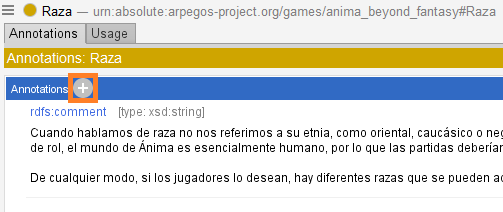
\includegraphics[scale=0.6]{Figures/Protege/UniqueSelection_1.png}
        \caption{Pulsar el botón “+” en el campo de anotaciones}.
        \label{UniqueSelection_1}
    \end{figure}

    \item Crear/Seleccionar el tipo de anotación \underline{ViewType} (Figura \ref*{UniqueSelection_2}).
    \begin{figure}[ht]
        \centering
        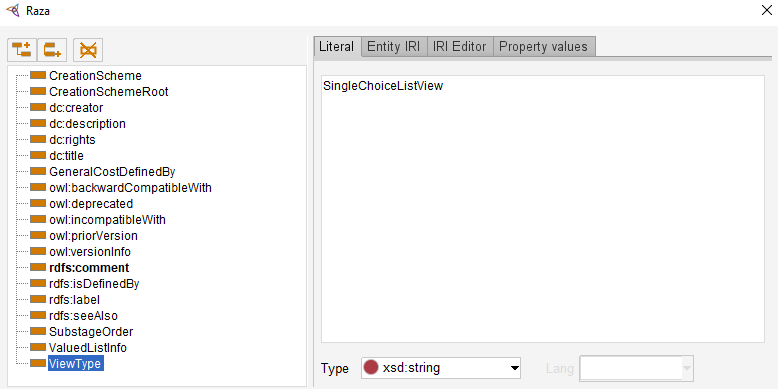
\includegraphics[scale=0.6]{Figures/Protege/UniqueSelection_2.png}
        \caption{Seleccionar el tipo de anotación \textit{ViewType}}.
        \label{UniqueSelection_2}
    \end{figure}

    \item Introducir como valor de la anotación el texto \underline{SingleChoiceListView}.
    \item Seleccionar como tipo de datos de la anotación \underline{xsd:string}.
    \item Pulsar el botón \textit{Aceptar}.
\end{enumerate}

\subsubsection{Etapa de selección múltiple}
La selección única es muy práctica, pero no resuelve los casos en los que es posible escoger más de una opción 
de un conjunto de posibilidades. Por ello se ha desarrollado otro tipo de etapa que permite abordar esta situación.\medskip

Este tipo de vista tiene algunas variaciones, que permiten a la aplicación adaptarse a cada caso según convenga.
En \anima se han encontrado tres de estas variaciones, asociadas principalmente al gasto de puntos:

\begin{itemize}
    \item \textit{Coste uniforme}: Todos los elementos tienen el mismo coste.
    \item \textit{Coste uniforme con coste de grupo}: Todos los elementos tienen el mismo coste, además de un coste por 
    abrir las opciones de un grupo.
    \item \textit{Coste heterogéneo}: Cada elemento tiene un coste distinto.
\end{itemize}

\subsubsection{Etapa de selección múltiple con coste uniforme} \label{MultipleChoiceStaticLimit}
Para el caso más simple, se utilizará como ejemplo la selección de \textit{Desventajas}. En \anima, un personaje sólo 
puede disponer de tres desventajas como máximo, así que cada opción tiene coste unitario (1). Como ya se han explicado 
previamente los procesos de creación de clases, individuos y propiedades, se pasará a explicar directamente cómo 
configurar la clase \textit{Desventaja} para ser una etapa de selección múltiple con coste uniforme.

\begin{enumerate}
    \item Acceder a la vista \textit{Classes} de la opción \textit{Entities}.
    \item Seleccionar la clase que se desea convertir en etapa.
    \item Añadir una anotación \underline{ViewType} con valor \underline{MultipleChoiceStaticLimitView} de tipo \textit{xsd:string}
    (Figura \ref*{MultipleChoice_1}).
    \begin{figure}[H]
        \centering
        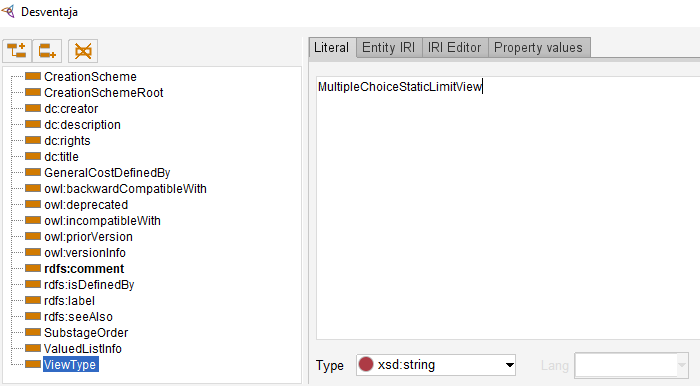
\includegraphics[scale=0.6]{Figures/Protege/MultipleChoice_1.png}
        \caption{Añadir anotación \textit{ViewType}}.
        \label{MultipleChoice_1}
    \end{figure}
\end{enumerate}

\subsubsection{Etapa de selección múltiple con coste uniforme y coste de grupo}\label{MultipleChoiceUniformCostGroup}
Esta versión es muy parecida a la anterior. La única diferencia es que para poder seleccionar un elemento de un grupo, hay que pagar 
un coste. Un caso de este tipo sucede en los poderes psíquicos de \anima, ya que para poder optar a una disciplina psíquica, es 
necesario pagar un consumo de voluntad (CV), y hay que pagar otro por cada poder elegido de dicha disciplina.\medskip

En este caso, antes de empezar a explicar el proceso, es importante aclarar cómo se conforman los grupos. La clase \textit{Poder Psíquico}
no tiene individuo alguno, sino que está formada por subclases, donde cada una de ellas representa un grupo, que aplicado al ejemplo, 
representan cada \textit{Disciplina Psíquica} disponible en el juego. Son los grupos los que contienen los diversos individuos, 
y los grupos tienen como clase padre aquella que representa la etapa (Figura \ref*{Groups}).

\begin{figure}[H]
    \centering
    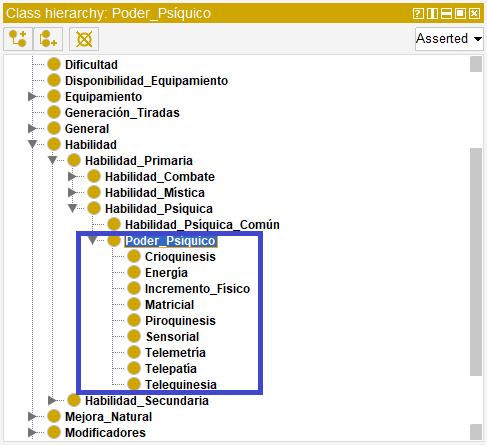
\includegraphics[scale=0.6]{Figures/Protege/Groups.png}
    \caption{Ejemplo de creación de grupos en una etapa}.
    \label{Groups}
\end{figure}

\begin{enumerate}
    \item Seguir los pasos del apartado \ref*{MultipleChoiceStaticLimit}, introduciendo como valor de la anotación \textit{ViewType}
    el valor \underline{MultipleChoiceStaticLimitGroupCostView}.
    \item Seleccionar la clase que representa a la etapa en la jerarquía de la vista \textit{Classes} de la opción \textit{Entities}.
    \item La etapa de ejemplo requiere un límite específico. Para ello se deben seguir las indicaciones del 
    apartado \nameref{SpecificLimit}.
\end{enumerate}

\subsubsection{Etapa de selección múltiple con coste heterogéneo}
En esta variante, cada elemento disponible en la selección tiene un valor característico. Un ejemplo de este caso puede ser la 
selección de \textit{Habilidades del Ki}. Cada habilidad de Ki tiene asociado su propio coste, de manera que este puede coincidir 
o no con el coste de otras habilidades. Esta etapa se construye utilizando el mismo método que en el apartado \ref*{MultipleChoiceUniformCostGroup}
, pero en la anotación \textit{ViewType} hay que introducir el texto \underline{MultipleChoiceDynamicLimitView}. Además, cada individuo 
debe tener indicado su coste con una propiedad de datos cuyo nombre siga la estructura \textit{Etapa\_Coste} (Figura ).

\begin{figure}[H]
    \centering
    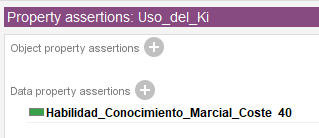
\includegraphics[scale=0.6]{Figures/Protege/Coste_seleccion_individuo.png}
    \caption{Coste de selección de un individuo}.
    \label{Coste_seleccion_individuo}
\end{figure}

\subsubsection{Etapa de introducción de valores}
Esta es la etapa más compleja, pues en ella el usuario tiene que indicar directamente los puntos que desea gastar en cada una 
de las opciones que se muestran. Es necesario resaltar que en esta etapa, el valor de los puntos gastados no coincide generalmente 
con el valor de la habilidad, sino que al valor introducido por el usuario se le aplican modificadores (indicados por el juego) para 
calcular el valor total de la habilidad. Como ejemplo se tratará el caso de las \textit{Habilidades de Combate de tipo común} de \anima, 
que son las habilidades físicas de ataque y defensa de un personaje:

\begin{enumerate}
    \item Seleccionar la clase que será reconocida como etapa en la vista \textit{Classes} de la opción \textit{Entities}.
    \item Añadir una anotación de tipo \textit{ViewType} con el texto \underline{ValuedViewList}.
    \item Añadir una anotación de tipo \textit{ValuedListInfo}. Para saber como crear esta anotación, 
    leer el apartado \nameref{ValuedListInfo} (Figura \ref*{ValuedListInfo_End}).

    \begin{figure}[H]
        \centering
        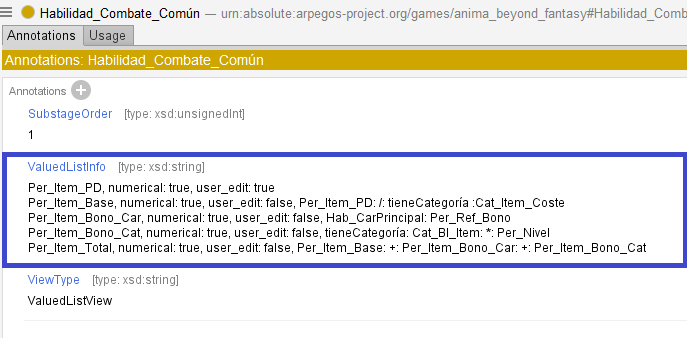
\includegraphics[scale=0.6]{Figures/Protege/ValuedListInfo_End.png}
        \caption{Crear una anotación de tipo \textit{ValuedListInfo}}.
        \label{ValuedListInfo_End}
    \end{figure}
\end{enumerate}

\subsubsection{Etapa raíz de creación}
La etapa raíz de creación es aquella que determina cuáles son los pasos que debe seguir el sistema durante el proceso 
de creación de un personaje. Se podría decir que esta etapa debe ser aquella que define el tipo de personaje. En el 
caso de \anima, se considera como etapa raíz de creación la selección de \textit{Categoría}, pues no todas las categorías 
tienen que recorrer todas las etapas de creación. \medskip

\begin{enumerate}
    \item Seleccionar la clase que será reconocida como etapa raíz en la vista \textit{Classes} de la opción \textit{Entities}.
    \item Añadir una anotación de tipo \textit{CreationSchemeRoot} con valor \textit{true} y tipo de datos 
    \textit{xsd:boolean} (Figura \ref*{CreationSchemeRoot}).

    \begin{figure}[H]
        \centering
        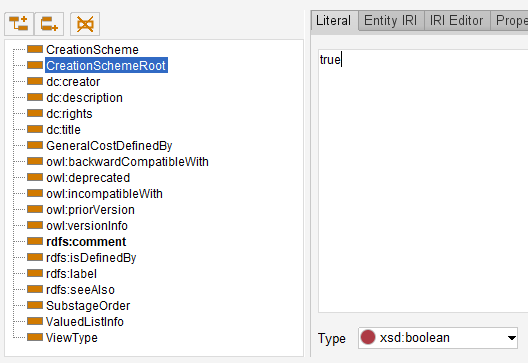
\includegraphics[scale=0.6]{Figures/Protege/CreationSchemeRoot.png}
        \caption{Crear una anotación de tipo \textit{CreationSchemeRoot}}.
        \label{CreationSchemeRoot}
    \end{figure}

    \item En cada individuo de esta clase, añadir una anotación de tipo \textit{CreationScheme} en la que 
    están dispuestos los nombres ordenados de las etapas que tiene que seguir el proceso de creación en caso de 
    seleccionar ese individuo. Los nombres de las etapas deben estar separados por comas (,), tal y como muestra 
    la figura \ref*{CreationScheme}.

    \begin{figure}[H]
        \centering
        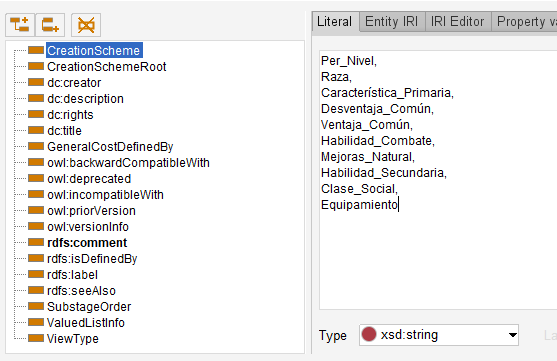
\includegraphics[scale=0.6]{Figures/Protege/CreationScheme.png}
        \caption{Crear una anotación de tipo \textit{CreationScheme} ne cada individuo de la etapa raíz}.
        \label{CreationScheme}
    \end{figure}
\end{enumerate}

\subsection{Configuración avanzada}
A continuación se describen algunos elementos que pueden ser requeridos por las etapas de creación, en función del juego de rol y 
de su proceso de creación de personaje.

\subsubsection{Crear una anotación de tipo \textit{ValuedListInfo}}\label{ValuedListInfo}
Esta anotación es muy especial, pues no sólo indica los diferentes valores y modificadores que debe tener cada individuo de la etapa, 
sino que además indica cómo deben calcularse, de manera que se pueda obtener el valor final de cada individuo. Un ejemplo de 
esta anotación puede apreciarse en la figura \ref*{ValuedListInfo_Begin}\medskip

\begin{figure}[H]
    \centering
    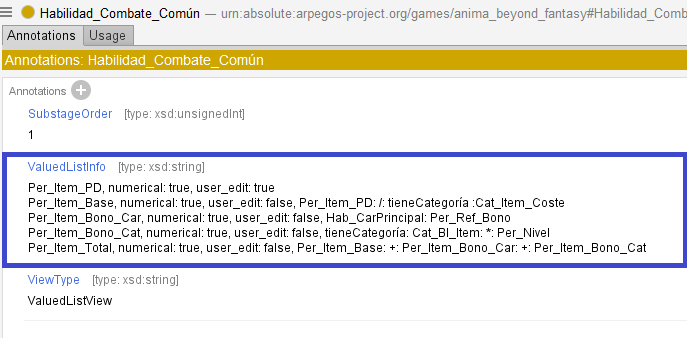
\includegraphics[scale=0.6]{Figures/Protege/ValuedListInfo_End.png}
    \caption{Anotación de tipo\textit{ValuedListInfo}}.
    \label{ValuedListInfo_Begin}
\end{figure}

La anotación \textit{ValuedListInfo} está compuesta por filas, donde cada una de ellas representa una propiedad de datos 
de un individuo de la etapa. Esto quiere decir que cada individuo de la etapa debe tener obligatoriamente una propiedad 
de datos por cada fila existente en esta anotación. El tipo de datos de esta anotación debe ser \textit{xsd:string}. \medskip

A su vez, cada fila está separada en cuatro campos, ordenados de izquierda a derecha:
\begin{enumerate}
    \item \textit{Nombre de la propiedad}: Este campo debe contener el nombre de la propiedad a la que se refiere.
    \item \textit{Numerical}: Indica si la propiedad de datos utiliza un valor numérico. Debe ir acompañada de las opciones 
    \textit{true} o \textit{false} separadas por dos puntos (:). La opción \textit{true} indicará que es un valor numérico, 
    mientra que la opción\textit{false} indicará que no se trata de un valor numérico.
    \item \textit{User\_edit}: Este campo indica si el valor de la propiedad de datos lo edita el usuario manualmente, o si 
    debe ser calculado por el sistema. Debe ir acompañada de una de las opciones \textit{true} o \textit{false} 
    separadas por dos puntos (:). La opción \textit{true} indicará que el usuario es quien introduce el valor, mientras que 
    la opción \textit{false} indicará que el valor debe ser calculado por el sistema.
    \item \textit{Formula}: Este campo indica la fórmula de cálculo del valor de la propiedad de datos, en caso de que no 
    no sea el usuario quien introduzca el valor manualmente.
\end{enumerate}

Una de las características que deben ser resaltadas, es que los nombres de las propiedades contienen la palabra \textit{Item}.
Cuando el sistema procesa una anotación de este tipo, sustituye la palabra \underline{Item} por el nombre del individuo cuyo valor se 
está procesando. Esto quiere decir que la propiedad \textit{Per\_Item\_PD} que aparece en la figura \ref*{ValuedListInfo_Begin}, 
se llamará \textit{Per\_Ataque\_PD} para la habilidad de ataque, mientras que para la habilidad de esquiva deberá llamarse 
\textit{Per\_Esquiva\_PD}. \medskip

El campo \textit{Formula} requiere algo más de atención, pues es necesario seguir unas normas a la hora de crear una fórmula 
para que ésta funcione correctamente:

\begin{itemize}
    \item Los elementos de la fórmula se separarán mediante el carácter de dos puntos (:).
    
    \item Para referirse a una propiedad de datos mencionada previamente en la anotación, basta con indicar el nombre de la 
    propiedad tal y como está indicado en la anotación. En la figura \ref*{ValuedListInfo_Begin} se puede observar que 
    en la segunda fila, para hacer referencia al valor de la primera propiedad, se introduce en la fórmula el valor del 
    primer campo de la primera fila (\textit{Per\_Item\_PD}).

    \item Para referirse a una propiedad de datos de un individuo diferente, hay que indicar en primer lugar la propiedad 
    de objeto por la que el personaje se relaciona con ese individuo, y a continuación, separado por dos puntos (:), indicar 
    el nombre de la propiedad de datos deseada. En la figura \ref*{ValuedListInfo_Begin} se puede apreciar que en la segunda 
    fila, se hace referencia a una propiedad de coste referente a la categoría del personaje (\textit{Cat\_Item\_Coste}).
    Para poder acceder a esta propiedad, es necesario conocer la categoría del personaje, por lo que previamente se utiliza 
    la propiedad de objeto \textit{tieneCategoría}, lo que hace que \textit{Item} se sustituya por el nombre del individuo que 
    representa la categoría del personaje. Así, para poder utilizar el valor de (\textit{Cat\_Item\_Coste}), es necesario introducirlo 
    de la siguiente manera en la fórmula: \textit{tieneCategoría:Cat\_Item\_Coste}. \textbf{Importante}: Esto se puede aplicar tanto 
    a propiedades de datos como a propiedades de objeto.

    \item Para realizar operaciones entre las propiedades de las fórmulas, basta con introducir el signo de la operación entre ambas 
    propiedades, separado de ambas mediante dos puntos (:). En la figura \ref*{ValuedListInfo_Begin} se puede contemplar que en la 
    segunda fila se utiliza el operador de división (/) entre las propiedades \textit{Per\_Item\_PD} y 
    \textit{tieneCategoría:Cat\_Item\_Coste}, siendo \textit{Per\_Item\_Base} el resultado de dividir el valor de la propiedad 
    \textit{Per\_Item\_PD} entre el valor de la propiedad \textit{tieneCategoría:Cat\_Item\_Coste}.

    \item En caso de que el valor de una propiedad de datos forme parte del nombre de una propiedad de la fórmula, hay que 
    buscar el valor de la primera mediante la formula y a continuación llamar a la segunda sustituyendo la posición donde 
    iría el valor numérico por la cadena de texto \underline{Ref}. Un ejemplo de este uso se muestra en la figura \ref*{Ref_example}.

    \item La aplicación no reconocerá el uso de paréntesis para los cálculos, de modo que hay que indicar todas las operaciones siguiendo 
    un orden estricto de izquierda a derecha.

    \begin{figure}[H]
        \centering
        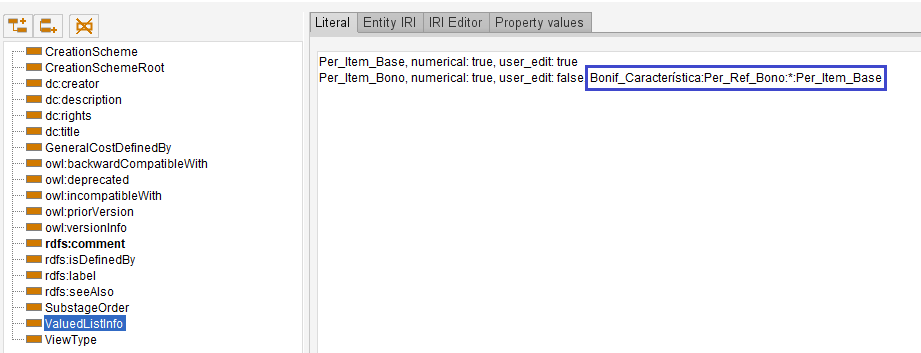
\includegraphics[scale=0.6]{Figures/Protege/Ref_example.png}
        \caption{Ejemplo de uso de la cadena de texto \textit{Ref} en una anotación de tipo \textit{ValuedListInfo}}.
        \label{Ref_example}
    \end{figure}
\end{itemize}

Siguiendo estas normas, no debería tener problema alguno para desarrollar su propia anotación de tipo \textit{ValuedListInfo}.
En caso de duda, no dude en consultar la ontología de ejemplo, pues todos los casos diseñados parten de las necesidades de 
esta ontología.

\subsubsection{Añadir un límite general de puntos a una etapa de creación}\label{GeneralLimit}
Algunas etapas de creación requieren la disposición de un límite de puntos que se pueden gastar en ellas. A continuación
se muestra el método para introducir un límite en una etapa de creación:

\begin{enumerate}
    \item Acceder a la vista \textit{Data Properties}
    \item Crear una propiedad de datos \textit{Etapa\_Límite} con la clase de la etapa como dominio y tipo de valor 
    \textit{xsd:unsignedInt} (Figura \ref*{MultipleChoice_2}).
    \begin{figure}[H]
        \centering
        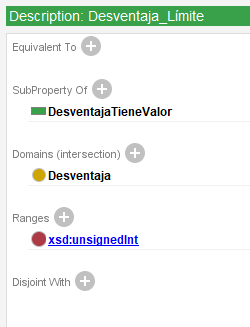
\includegraphics[scale=0.6]{Figures/Protege/MultipleChoice_2.png}
        \caption{Crear propiedad \textit{Etapa\_Límite}}.
        \label{MultipleChoice_2}
    \end{figure}
    \item Crear anotación \textit{rdfs:IsDefinedBy} con el valor límite de la propiedad \textit{Etapa\_Límite} 
    (Figura \ref*{MultipleChoice_3} ). En caso de que el límite sea el valor de otra propiedad de datos, indicar 
    el nombre de la propiedad de manera exacta (Figura \ref*{MultipleChoice_4}).
    \begin{figure}[H]
        \centering
        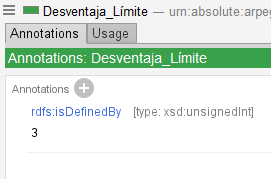
\includegraphics[scale=0.6]{Figures/Protege/MultipleChoice_3.png}
        \caption{Crear anotación \textit{IsDefinedBy} con valor numérico}.
        \label{MultipleChoice_3}
    \end{figure}
    \begin{figure}[H]
        \centering
        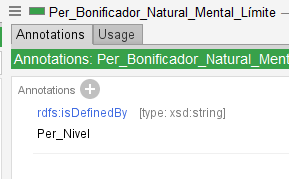
\includegraphics[scale=0.6]{Figures/Protege/MultipleChoice_4.png}
        \caption{Crear anotación \textit{IsDefinedBy} con referencia a otra propiedad}.
        \label{MultipleChoice_4}
    \end{figure}
\end{enumerate}

\subsubsection{Añadir un límite específico de puntos a una etapa de creación}\label{SpecificLimit}
En algunos casos es necesario añadir un límite distinto al establecido por el método anterior, ya sea porque la etapa tenga varios 
límites, o porque sea necesario limitar otro tipo de puntos. Un buen ejemplo para este caso son los poderes psíquicos en \anima, 
puesto que los poderes psíquicos no gastan \textit{puntos de desarrollo} como el resto de habilidades, sino que gastan 
\textit{Consumos de Voluntad}, por lo que el límite de puntos de desarrollo no resulta útil en este caso.\medskip

Para declarar este nuevo límite, 
hay que añadir una anotación \underline{GeneralCostDefinedBy} indicando el valor o la propiedad que indica el 
límite de puntos a gastar en la etapa (Figura \ref*{MultipleChoiceGroupCost_1}).

\begin{figure}[H]
    \centering
    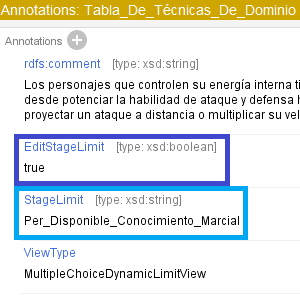
\includegraphics[scale=0.6]{Figures/Protege/MultipleChoiceGroupCost_1.png}
    \caption{Añadir anotación \textit{GeneralCostDefinedBy}}.
    \label{MultipleChoiceGroupCost_1}
\end{figure}

\subsubsection{Añadir un elemento específico en una etapa}
En algunos casos, es posible que una etapa de creación requiera que el usuario seleccione (o introduzca el valor de) un elemento 
que se tiene en consideración más adelante. En \anima este caso se da, por ejemplo, con el \textit{Conocimiento Marcial}, que es 
una "habilidad" cuyo valor se utiliza como límite para algunas habilidades de combate, como las artes marciales. 
En estos casos, hay que llevar a cabo los siguientes pasos:

\begin{enumerate}
    \item Seleccionar la clase que representa la etapa que utiliza el elemento que se desea introducir 
    (en la vista \textit{Classes} de la opción \textit{Entities}).
    \item Crear una subclase de la clase seleccionada para introducir el elemento específico de la etapa 
    (Figura \ref*{ElementoComun_1}).
    \begin{figure}[H]
        \centering
        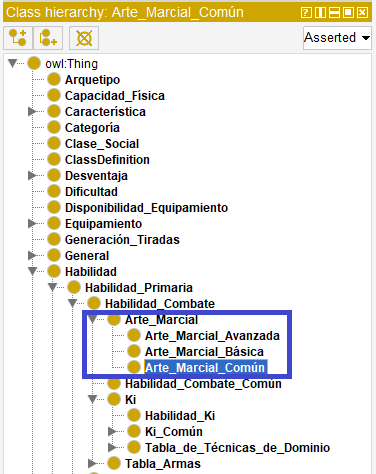
\includegraphics[scale=0.6]{Figures/Protege/ElementoComun_1.png}
        \caption{Crear subclase para el elemento específico}.
        \label{ElementoComun_1}
    \end{figure}

    \item Convertir la subclase en una etapa de creación, cuyo tipo depende de la interacción requerida por el elemento específico.
    \item Añadir a la subclase recién creada una anotación de tipo \textit{SubstageOrder}, ubicando esta subclase en un puesto 
    anterior que aquellas que requieren el uso del elemento específico (Figura \ref*{ElementoComun_2}).
    \begin{figure}[H]
        \centering
        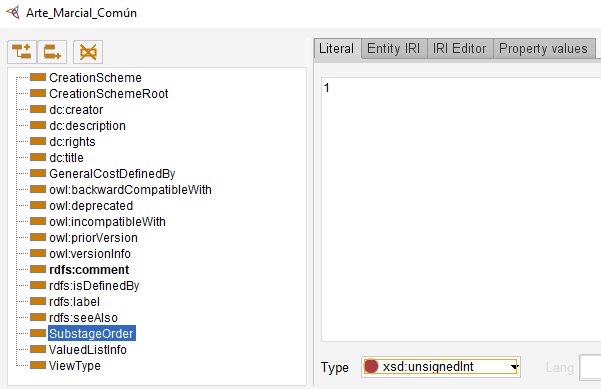
\includegraphics[scale=0.6]{Figures/Protege/ElementoComun_2.png}
        \caption{Crear subclase para el elemento específico}.
        \label{ElementoComun_2}
    \end{figure}

\end{enumerate}

\subsubsection{Añadir un requisito a un individuo}
En los juegos de rol es algo natural que haya elementos que tengan requisitos, de manera que resulte imposible de utilizar si 
el personaje no supera correctamente estas condiciones. Hay dos tipos de requisitos: requisitos de objeto, En los requisitos de objeto, 
en los que el elemento simplemente necesita que se cumpla una propiedad de objeto, y los requisitos de dato, que son aquellos en los que 
propiedad indicada debe superar el valor establecido por el requisito. El mejor ejemplo de esto en \anima son las 
\textit{Artes Marciales Avanzadas}. Estas habilidades tienen múltiples requisitos, que además suelen ser muy costosos, 
lo que hace difícil poder acceder a ellas. \medskip 

Lo que el equipo de desarrollo recomienda es crear un conjunto de propiedades que representen requisitos de objeto y de datos, 
y que se utilicen tantas como requisitos tenga cada individuo. Las propiedades de requisitos deben nombrarse de la siguiente manera:
\begin{itemize}
    \item \textbf{Requisito de objeto}: \textit{Clase\_RequisitoClave\_x}, donde \textit{x} representa la posición ordinal del requisito.
    \item \textbf{Requisito de datos}: \textit{Clase\_RequisitoValor\_x}.
\end{itemize}

Por cada requisito de datos, debe utilizarse una propiedad de cada tipo: la propiedad \textit{RequisitoClave} indica el nombre de la 
propiedad que debe superar el valor establecido, y la propiedad \textit{RequisitoValor} indica la puntuación mínima que hay que 
superar para dar el requisito por satisfecho.\medskip

Para crear un requisito de objeto, hay que seguir los siguientes pasos:
\begin{enumerate}
    \item Asociar al individuo que tiene el requisito una propiedad de objeto de tipo \textit{Clase\_RequisitoClave\_x}, en la que se 
    debe introducir como valor el nombre de la propiedad requerida.
\end{enumerate}

Un requisito de datos tiene que crearse de la siguiente manera:
\begin{enumerate}
    \item Asociar al individuo una propiedad de objeto de tipo \textit{Clase\_RequisitoClave\_x}, en la que se 
    debe introducir como valor el nombre de la propiedad requerida.
    \item Asociar al individuo una propiedad de datos \textit{Clase\_RequisitoValor\_x}, que debe tener 
    como valor el mínimo necesario para que se pueda considerar que el usuario supera el requisito. En este caso, el valor \textit{x}
    debe ser el mismo en ambas propiedades.
\end{enumerate}

En la figura \ref*{requisitos} se pueden observar estos requisitos aplicados a un \textit{Arte Marcial Avanzada} de \anima.

\begin{figure}[ht]
    \centering
    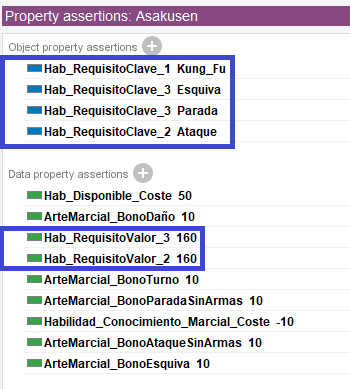
\includegraphics[scale=0.6]{Figures/Protege/Requisitos.png}
    \caption{Requisitos de un individuo}.
    \label{requisitos}
\end{figure}

\subsubsection{Indicar el orden de una subetapa}
Algunas etapas de creación están compuestas de un conjunto de etapas de distinto tipo, y por esto, no se pueden abordar todas igual.
Estas etapas requieren de algún tipo de ordenamiento, pues no se pueden mostrar todas a la vez. Para indicar el orden de estas subetapas
hay que añadir a cada subetapa una anotación de tipo \textit{SubstageOrder}, introduciendo un número positivo indicando su posición 
y con el tipo de datos \textit{xsd:unsignedInt}, como se muestra en la figura \ref*{SubstageOrder}.

\begin{figure}[ht]
    \centering
    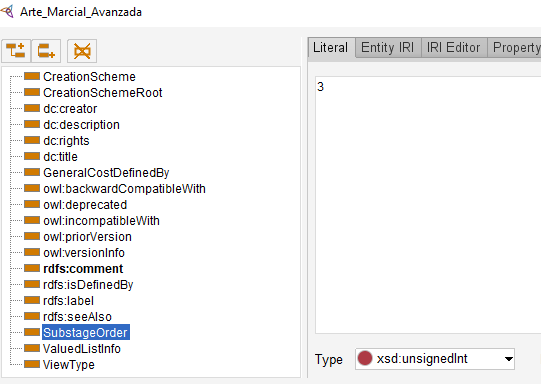
\includegraphics[scale=0.6]{Figures/Protege/SubstageOrder.png}
    \caption{Requisitos de un individuo}.
    \label{SubstageOrder}
\end{figure}

